\section{Eigenwerte}

\subsection{Theorie}

\begin{bonus}{Wiederholung Eigenwerte}
    Es gilt:
    \begin{itemize}
        \item $A \in \R^{n \times n}$ hat \emph{Eigenwerte} $\lambda$, falls
              \[
                  \det(A - \lambda I) = p_A(\lambda) = 0
              \]
              d. h. falls $\lambda$ Nullstelle des \emph{charakteristischen Polynoms} $p_A$ ist
        \item $p_A$ hat Grad $n$,
              \[
                  p_A(\lambda) = c \cdot (\lambda - \lambda_1) \cdot \ldots \cdot (\lambda - \lambda_n), \quad \lambda_1, \ldots, \lambda_n \in \C
              \]
        \item ist $\lambda_i = \lambda_j$, $i \neq j$, so heißt $\lambda_i$ \emph{mehrfacher Eigenwert}
        \item $v_i \in \R^n$ ist Eigenvektor von $A$ zu $\lambda_i$, falls $v_i \neq 0$, $A v_i = \lambda_i v_i$
        \item ist $v_i \in \R^n$ Eigenvektor zu $\lambda_i$, dann ist auch $c \cdot v_i$ Eigenvektor zu $\lambda_i$ ($c \neq 0$)
        \item bei mehrfachen Eigenwerten unterscheidet man die \emph{algebraische Vielfachheit}\footnote{d.h. die Vielfachheit der Nullstelle im charakteristischen Polynom $p_A$}, und die \emph{geometrische Vielfachheit}\footnote{d.h. die Anzahl der linear unabhängigen Eigenvektoren zu dem mehrfachen Eigenwert}
              \begin{itemize}
                  \item für beide Werte gilt der Zusammenhang:
                        \[
                            1 \leq \ \text{geometrische Vielfachheit} \ \leq \ \text{algebraische Vielfachheit}
                        \]
              \end{itemize}
        \item ist $A \in \R^{n \times n}$ und $T \in \R^{n \times n}$ regulär, dann haben $A$ und $TAT^{-1}$ die selben Eigenwerte
        \item besitzt $A$ $n$ linear unabhängige Eigenvektoren $v_i$ mit Eigenvektoren $\lambda_i$, dann gilt
              \[
                  A = T
                  \begin{pmatrix}
                      \lambda_1 &        &           \\
                                & \ddots &           \\
                                &        & \lambda_n
                  \end{pmatrix}
                  T^{-1}, \quad T =
                  \begin{pmatrix}
                      v_1 & \ldots & v_n
                  \end{pmatrix}
              \]
              d. h. $A$ ist \emph{diagonalisierbar}
    \end{itemize}
\end{bonus}

\begin{defi}{Satz von Gerschgorin}
    Sei $A \in \R^{n \times n}$ und
    \[
        K = \bigcup_{i = 1}^{n} K_i, \quad K_i = \{ z \mid z \in \C, |z - a_{ii}| \leq \sum_{j \neq i} | a_{ij} | \}
    \]

    Dann gilt für die Eigenwerte $\lambda_i$ von $A$, dass $\lambda_i \in K$ für alle $i$.
\end{defi}

\begin{example}{Satz von Gerschgorin}
    Gegeben sei eine Matrix $A$ mit
    \[
        A =
        \begin{pmatrix}
            3 & 1 & 1 \\
            0 & 2 & 0 \\
            1 & 0 & 1
        \end{pmatrix}
    \]

    Berechnen Sie die Eigenwerte von $A$ per Hand und wenden Sie dann den Satz von Gerschgorin auf $A$ und $A^T$ an.

    \exampleseparator

    \[
        p(\lambda) = \det(A - \lambda I) = \det
        \begin{pmatrix}
            3 - \lambda & 1           & 1           \\
            0           & 2 - \lambda & 0           \\
            1           & 0           & 1 - \lambda
        \end{pmatrix}
        = \ldots = (2 - \lambda) (\lambda^2 - 4\lambda + 2)
    \]
    % \begin{alignat*}{1}
    %     p(\lambda) = & \det(A - \lambda I)                                                  \\
    %     =            & \det
    %     \begin{pmatrix}
    %         3 - \lambda & 1           & 1           \\
    %         0           & 2 - \lambda & 0           \\
    %         1           & 0           & 1 - \lambda
    %     \end{pmatrix}                                                           \\
    %     =            & (2 - \lambda) \det
    %     \begin{pmatrix}
    %         3 - \lambda & 1           \\
    %         1           & 1 - \lambda
    %     \end{pmatrix}                                                           \\
    %     =            & (2 - \lambda) \left( (\lambda - 3) (\lambda - 1) - 1 \cdot 1 \right) \\
    %     =            & (2 - \lambda) (\lambda^2 - 4\lambda + 2)
    % \end{alignat*}
    \[
        p(\lambda) = 0 \quad \implies \lambda_1 = 2, \quad \lambda_{2, 3} = 2 \pm \sqrt{4 - 2} = 2 \pm \sqrt{2}
    \]

    Nach dem Satz von Gerschgorin gilt für $A$ bzw. $A^T$:
    \[
        A =
        \left(
        \begin{array}{ccc}
                \cellcolor{red!20} 3 & \cellcolor{red!10} 1 & \cellcolor{red!10} 1 \\
                \cellcolor{red!10} 0 & \cellcolor{red!20} 2 & \cellcolor{red!10} 0 \\
                \cellcolor{red!10} 1 & \cellcolor{red!10} 0 & \cellcolor{red!20} 1
            \end{array}
        \right)
        \quad \implies \quad
        \begin{matrix}
            \cellcolor{red!20} m_1 = 3 &  & \cellcolor{red!10} r_1 = |1| + |1| = 2 \\
            \cellcolor{red!20} m_2 = 2 &  & \cellcolor{red!10} r_2 = |0| + |0| = 0 \\
            \cellcolor{red!20} m_2 = 1 &  & \cellcolor{red!10} r_3 = |1| + |0| = 1
        \end{matrix}
    \]

    \begin{center}
        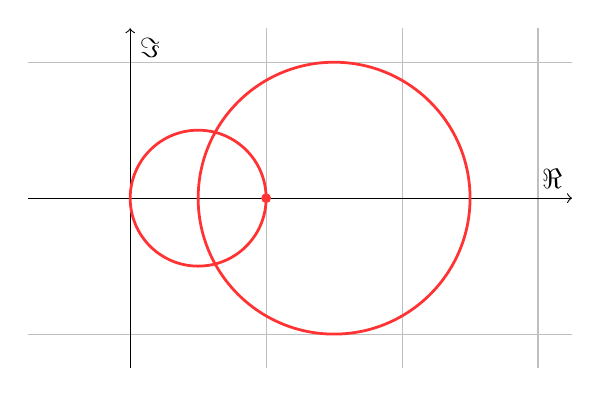
\begin{tikzpicture}
            \begin{axis}[
                    % xtick distance=2,
                    % ytick distance=2,
                    grid=major,
                    % grid style={line width=.1pt, draw=gray!10}%,major grid style={line width=.2pt,draw=gray!50}
                    ticks=none, % ticks aus?
                    axis lines = middle,
                    axis line style={->},
                    ymin=-2.5, ymax=2.5,
                    xmin=-1.5, xmax=6.5,
                    xlabel={$\Re$},
                    ylabel={$\Im$},
                    axis equal image,
                    width=0.7\textwidth
                ]
                \def\circlewidth{1pt}
                % A
                \draw[red!80, line width=\circlewidth] (axis cs:3,0) node[circle=2pt] {} circle (2);
                \draw[red!80, line width=\circlewidth, fill] (axis cs:2,0) circle (0.05);
                \draw[red!80, line width=\circlewidth] (axis cs:1,0) circle (1);

            \end{axis}
        \end{tikzpicture}
    \end{center}

    \[
        A^T =
        \left(
        \begin{array}{ccc}
                \cellcolor{red!20} 3 & \cellcolor{red!10} 0 & \cellcolor{red!10} 1 \\
                \cellcolor{red!10} 1 & \cellcolor{red!20} 2 & \cellcolor{red!10} 0 \\
                \cellcolor{red!10} 1 & \cellcolor{red!10} 0 & \cellcolor{red!20} 1
            \end{array}
        \right)
        \quad \implies \quad
        \begin{matrix}
            \cellcolor{red!20} m_1 = 3 &  & \cellcolor{red!10} r_1 = |0| + |1| = 1 \\
            \cellcolor{red!20} m_2 = 2 &  & \cellcolor{red!10} r_2 = |1| + |0| = 1 \\
            \cellcolor{red!20} m_2 = 1 &  & \cellcolor{red!10} r_3 = |1| + |0| = 1
        \end{matrix}
    \]

    \begin{center}
        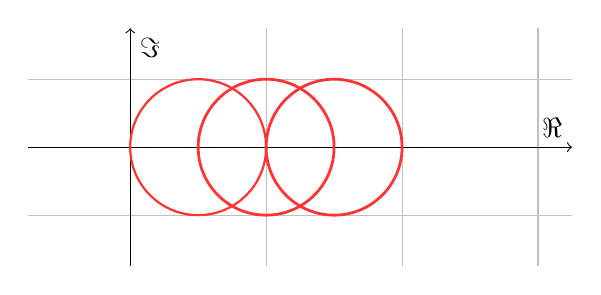
\begin{tikzpicture}
            \begin{axis}[
                    % xtick distance=2,
                    % ytick distance=2,
                    grid=major,
                    % grid style={line width=.1pt, draw=gray!10}%,major grid style={line width=.2pt,draw=gray!50}
                    ticks=none, % ticks aus?
                    axis lines = middle,
                    axis line style={->},
                    ymin=-1.75, ymax=1.75,
                    xmin=-1.5, xmax=6.5,
                    xlabel={$\Re$},
                    ylabel={$\Im$},
                    axis equal image,
                    width=0.7\textwidth
                ]
                \def\circlewidth{1pt}
                % A^T
                \draw[red!80, line width=\circlewidth] (axis cs:3,0) circle (1);
                \draw[red!80, line width=\circlewidth] (axis cs:2,0) circle (1);
                \draw[red!80, thick] (axis cs:1,0) circle (1);

            \end{axis}
        \end{tikzpicture}
    \end{center}
\end{example}

\begin{bonus}{Eigenwertproblem als Nullstellenproblem}
    Ist $A$ symmetrisch, so gelten zusätzlich folgende Aussagen:
    \begin{itemize}
        \item $\lambda_i \in \R, \forall i$
        \item es gibt $n$ Eigenvektoren $v_i$, die linear unabhängig sind, d.h. $A$ ist diagonalisierbar
        \item die $v_i$ können so gewählt werden, dass sie eine Orthonormalbasis bilden:
              \[
                  \langle v_i, v_j \rangle = \delta_{ij}, \quad i, j = 1, \ldots, n
              \]
        \item $Q = \begin{pmatrix}
                      v_1 & \ldots & v_n
                  \end{pmatrix}$ ist eine Orthonormalmatrix und es gilt:
              \[
                  A = Q \Lambda Q^{-1} = Q \Lambda Q^{T}, \quad \Lambda = \begin{pmatrix}
                      \lambda_1 &        &           \\
                                & \ddots &           \\
                                &        & \lambda_n
                  \end{pmatrix}
              \]
              bzw.
              \[
                  \Lambda = Q^T A Q
              \]
        \item da die $v_i$ eine Orthonormalbasis bilden, kann jeder Vektor $x \in \R^n$ geschrieben werden als
              \[
                  x = \sum_{i=1}^{n} x_i v_i, \quad x_i = \langle x, v_i \rangle
              \]
              und
              \[
                  Ax = \sum_{i=1}^{n} x_i A v_i = \sum_{i=1}^{n} \lambda_i x_i v_i
              \]
    \end{itemize}

    Das Eigenwertproblem ist also ein Nullstellenproblem für das Polynom $p_A$.

    Aus der Algebra wissen wir, dass es ab Polynomgrad 5 keinen endlichen Algorithmus zur Lösung dieses Problems gibt.
    Numerische Algorithmen können deswegen nur iterative Verfahren sein.
\end{bonus}

\subsection{Vektoriteration}

\begin{defi}{Vektoriteration}
    Die \emph{Vektoriteration} ist ein numerisches Verfahren zur Berechnung des betragsgrößten Eigenwertes und des dazugehörigen Eigenvektors einer Matrix.

    Wir wissen bereits, dass jedes $x \in \R^n$ als
    \[
        x = \sum_{i=1}^{n} x_i v_i, \quad x_i = \langle x, v_i \rangle
    \]
    geschrieben werden kann.
    Damit gilt:
    \[
        Ax = \sum_i \lambda_i x_i v_i \quad \implies \quad A^kx = \sum_i \lambda_i^k x_i v_i
    \]

    Gilt $|\lambda_1| > \dots > |\lambda_n|$, so dominiert der Anteil $\lambda_1 x_1 v_1$ (falls $x_1 \neq 0$) in $A^k x$.

    Wird $x$ oft genug mit $A$ multipliziert, so bleibt im wesentlichen ein Vielfaches von $v_1$ übrig.

    Ist $|\lambda_1| > 1$, so wird $\|A^kx\|_2$ immer größer.
    Um die damit verbundenen numerischen Probleme zu vermeiden normalisiert man nach jeder Multiplikation mit $A$ den neu berechneten Vektor und erhält somit die \emph{Vektoriteration}:
    \begin{enumerate}
        \item Wähle $x^{(0)}$ mit $\|x^{(0)}\|_2 = 1$ und $x_1^{(0)} = \langle x^{(0)}, v_1 \rangle \neq 0$
        \item Wiederhole:
              \[
                  y^{(k+1)} = A x^{(k)}
              \]
              \[
                  x^{(k+1)} = \frac{y^{(k+1)}}{ \| y^{(k+1)} \|_2 }
              \]
              \[
                  \mu^{(k+1)} = \langle x^{(k)}, y^{(k+1)} \rangle
              \]
    \end{enumerate}

    Ist $A$ symmetrisch mit $\lambda_1 > |\lambda_2| > \dots > |\lambda_n|$.
    Dann ist die Vektoriteration
    \[
        \mu^{(k)} \xrightarrow{k \to \infty} \lambda_1, \quad x^{(k)} \xrightarrow{k \to \infty} \sign(x_1^{(0)}) v_1
    \]
    falls $x_1^{(0)} = \langle x^{(0)}, v_1 \rangle \neq 0$ ist.
\end{defi}

\begin{example}{Vektoriteration}
    Gegeben seien eine Matrix $A$ und ein Startvektor $x^{(0)}$ mit:
    \[
        A =
        \begin{pmatrix}
            2 & 1 & 0 & 0 \\
            1 & 2 & 1 & 0 \\
            0 & 1 & 2 & 1 \\
            0 & 0 & 1 & 2
        \end{pmatrix}
        , \quad
        x^{(0)} =
        \begin{pmatrix}
            1 \\ 0 \\ 0 \\ 0
        \end{pmatrix}
    \]

    Wenden Sie die Vektoriteration an und berechnen Sie den betragsgrößten Eigenwert und den Eigenvektor.

    \exampleseparator

    $k = 1$:
    \[
        y^{(1)} = A x^{(0)} =
        \begin{pmatrix}
            2 & 1 & 0 & 0 \\
            1 & 2 & 1 & 0 \\
            0 & 1 & 2 & 1 \\
            0 & 0 & 1 & 2
        \end{pmatrix}
        \begin{pmatrix}
            1 \\ 0 \\ 0 \\ 0
        \end{pmatrix}
        =
        \begin{pmatrix}
            2 \\ 1 \\ 0 \\ 0
        \end{pmatrix}
    \]
    \[
        x^{(1)} = \frac{y^{(1)}}{ \| y^{(1)} \|_2 } = \frac{1}{\sqrt{5}}
        \begin{pmatrix}
            2 \\ 1 \\ 0 \\ 0
        \end{pmatrix}
        \approx
        \begin{pmatrix}
            0.89 \\ 0.45 \\ 0 \\ 0
        \end{pmatrix}
    \]
    \[
        \mu^{(1)} = \langle x^{(0)}, y^{(1)} \rangle = \langle
        \begin{pmatrix}
            1 \\ 0 \\ 0 \\ 0
        \end{pmatrix},
        \begin{pmatrix}
            2 \\ 1 \\ 0 \\ 0
        \end{pmatrix}
        \rangle
        = 2
    \]

    $k = 2$:
    \[
        y^{(2)} = A x^{(1)} = \frac{1}{\sqrt{5}}
        \begin{pmatrix}
            2 & 1 & 0 & 0 \\
            1 & 2 & 1 & 0 \\
            0 & 1 & 2 & 1 \\
            0 & 0 & 1 & 2
        \end{pmatrix}
        \begin{pmatrix}
            2 \\ 1 \\ 0 \\ 0
        \end{pmatrix}
        = \frac{1}{\sqrt{5}}
        \begin{pmatrix}
            5 \\ 4 \\ 1 \\ 0
        \end{pmatrix}
    \]
    \[
        x^{(2)} = \frac{y^{(2)}}{ \| y^{(2)} \|_2 } = \frac{1}{\sqrt{\frac{42}{5}}} \cdot \frac{1}{\sqrt{5}}
        \begin{pmatrix}
            5 \\ 4 \\ 1 \\ 0
        \end{pmatrix}
        = \frac{1}{\sqrt{42}}
        \begin{pmatrix}
            5 \\ 4 \\ 1 \\ 0
        \end{pmatrix}
        \approx
        \begin{pmatrix}
            0.77 \\ 0.62 \\ 0.15 \\ 0
        \end{pmatrix}
    \]
    \[
        \mu^{(2)} = \langle x^{(1)}, y^{(2)} \rangle = \frac{1}{5} \langle
        \begin{pmatrix}
            2 \\ 1 \\ 0 \\ 0
        \end{pmatrix},
        \begin{pmatrix}
            5 \\ 4 \\ 1 \\ 0
        \end{pmatrix}
        \rangle
        = 2.8
    \]

    $\ldots$

    $k = 15$:
    \[
        x^{(15)} \approx
        \begin{pmatrix}
            0.3793 \\ 0.6061 \\ 0.5968 \\ 0.3641
        \end{pmatrix}
        , \quad
        \mu^{(15)} \approx 3.6177
    \]
\end{example}

\subsection{Jacobi-Verfahren}

\begin{defi}{Jacobi-Verfahren (Eigenwerte)}
    Die Idee des \emph{Jacobi-Verfahrens} besteht darin, das jeweils betragsgrößte Außerdiagonalelement mit Hilfe einer Givens-Rotation auf $0$ zu bringen, und sich auf diese Art mehr und mehr einer Diagonalmatrix anzunähern.

    Es ergibt sich die Iterationsvorschrift:
    \begin{enumerate}
        \item $A^{0} = A$
        \item Wiederhole:
              \[
                  A^{(k+1)} = {Q^{(k)}}^T A^{(k)} Q^{(k)} = \underbrace{Q_k^T \cdot \ldots \cdot Q_1^T}_{{Q^{(k)}}^T} A^{(0)} \underbrace{Q_1 \cdot \ldots \cdot Q_k}_{Q^{(k)}}
              \]
              $Q_k$ wird wie folgt bestimmt:
              \begin{itemize}
                  \item suche das betragsgrößte Nebendiagonalelement $a_{i_0 j_0}^{(k-1)}$ von $A^{k-1}$
                  \item dabei kann $j_0 > i_0$ angenommen werden, da alle Matrizen $A^{k-1}$ symmetrisch sind
                  \item bestimme $Q_k$ so, dass $a_{i_0 j_0}^{(k)} = 0$, also
                        \[
                            Q_k =
                            \begin{pmatrix}
                                1 &        &   &    &   &        &   &   &   &        &   \\
                                  & \ddots &   &    &   &        &   &   &   &        &   \\
                                  &        & 1 &    &   &        &   &   &   &        &   \\
                                  &        &   & c  &   &        &   & s &   &        &   \\
                                  &        &   &    & 1 &        &   &   &   &        &   \\
                                  &        &   &    &   & \ddots &   &   &   &        &   \\
                                  &        &   &    &   &        & 1 &   &   &        &   \\
                                  &        &   & -s &   &        &   & c &   &        &   \\
                                  &        &   &    &   &        &   &   & 1 &        &   \\
                                  &        &   &    &   &        &   &   &   & \ddots &   \\
                                  &        &   &    &   &        &   &   &   &        & 1
                            \end{pmatrix}
                        \]
                        mit
                        \[
                            \alpha = \frac{a_{j_0 j_0} - a_{i_0 i_0}}{2 a_{i_0 j_0}} \quad \implies \quad c = \sqrt{\frac{1}{2} + \frac{1}{2} \sqrt{\frac{\alpha^2}{1 + \alpha^2}}}, \quad s = \frac{\sign(\alpha)}{2c \sqrt{1 + \alpha^2}}
                        \]
              \end{itemize}
    \end{enumerate}

    Dann ist ($\lambda_i$ Eigenwerte, $v_i$ Eigenvektoren)
    \[
        \diagonal(A^{(k)}) =
        \begin{pmatrix}
            a_{11}^{(k)} &        &              \\
                         & \ddots &              \\
                         &        & a_{nn}^{(k)}
        \end{pmatrix}
        \approx
        \begin{pmatrix}
            \lambda_1 &        &           \\
                      & \ddots &           \\
                      &        & \lambda_n
        \end{pmatrix}
        = \Lambda
    \]
    \[
        Q^{(k)} \approx
        \begin{pmatrix}
            v_1 & \ldots & v_n
        \end{pmatrix}
    \]
\end{defi}

\begin{example}{Jacobi-Verfahren}
    Gegeben sei die Matrix $A$ mit:
    \[
        A =
        \begin{pmatrix}
            3 & 4 \\
            4 & 3
        \end{pmatrix}
    \]

    Führen Sie das Jacobi-Verfahren für eine Iteration aus und berechnen Sie die Eigenwerte (näherungsweise).

    \exampleseparator

    \[
        A = A^{(0)} =
        \left(
        \begin{array}{cc}
                3 & \cellcolor{red!20} 4 \\
                4 & 3
            \end{array}
        \right)
        \quad \implies \quad
        i_0 = 1, \quad j_0 = 2
    \]

    Damit gilt:
    \[
        Q_1 =
        \begin{pmatrix}
            c  & s \\
            -s & c
        \end{pmatrix}
    \]
    mit
    \[
        \alpha = \frac{a_{j_0 j_0} - a_{i_0 i_0}}{2 a_{i_0 j_0}} = \frac{a_{22} - a_{11}}{2 a_{1 2}} = \frac{3 - 3}{2 \cdot 4} = 0
    \]
    \[
        \implies \quad c = \sqrt{\frac{1}{2} + \frac{1}{2} \sqrt{\frac{\alpha^2}{1 + \alpha^2}}} = \sqrt{\frac{1}{2}} = \frac{1}{\sqrt{2}}, \quad s = \frac{\sign(\alpha)}{2c \sqrt{1 + \alpha^2}} = \frac{1}{2 \cdot \frac{1}{\sqrt{2}} \cdot \sqrt{1}} = \frac{1}{\sqrt{2}}
    \]
    \[
        \implies \quad Q_1 =
        \left(
        \begin{array}{cc}
                \cellcolor{red!10} \nicefrac{1}{\sqrt{2}}  & \cellcolor{blue!10} \nicefrac{1}{\sqrt{2}} \\
                \cellcolor{red!10} -\nicefrac{1}{\sqrt{2}} & \cellcolor{blue!10} \nicefrac{1}{\sqrt{2}}
            \end{array}
        \right)
    \]
    \[
        \implies \quad A^{(1)} = Q_1^T A^{(0)} Q_1 =
        \begin{pmatrix}
            \nicefrac{1}{\sqrt{2}} & -\nicefrac{1}{\sqrt{2}} \\
            \nicefrac{1}{\sqrt{2}} & \nicefrac{1}{\sqrt{2}}
        \end{pmatrix}
        \begin{pmatrix}
            3 & 4 \\
            4 & 3
        \end{pmatrix}
        \begin{pmatrix}
            \nicefrac{1}{\sqrt{2}}  & \nicefrac{1}{\sqrt{2}} \\
            -\nicefrac{1}{\sqrt{2}} & \nicefrac{1}{\sqrt{2}}
        \end{pmatrix}
        = \ldots =
        \left(
        \begin{array}{cc}
                \cellcolor{red!20} -1 & 0                     \\
                0                     & \cellcolor{blue!20} 7
            \end{array}
        \right)
    \]

    Damit erhalten wir die Eigenwerte und dazugehörigen Eigenvektoren:
    \[
        \lambda_1 = -1, \quad v_1 =
        \begin{pmatrix}
            \nicefrac{1}{\sqrt{2}} \\ -\nicefrac{1}{\sqrt{2}}
        \end{pmatrix}
    \]
    \[
        \lambda_2 = 7, \quad v_2 =
        \begin{pmatrix}
            \nicefrac{1}{\sqrt{2}} \\ \nicefrac{1}{\sqrt{2}}
        \end{pmatrix}
    \]
\end{example}

\subsection{QR-Verfahren, Hessenberg-Transformation, Shift-Technik}

\begin{defi}{QR-Verfahren (singuläre Matrizen)}
    Mit Givens- bzw. Householder-Transformationen können wir eine \emph{reguläre Matrix} $A$ in $A = QR$ zerlegen, wobei $Q$ orthonormal und $R$ eine obere Dreiecksmatrix ist.

    Eine analoge Zerlegung ist auch für \emph{singuläres} $A$ möglich:
    \begin{itemize}
        \item Falls eine Spalte inklusive des Diagonalelements gleich $0$ ist, benutzt man als Dreh- bzw. Spiegelmatrix $Q_k = I$.
        \item Auf der Diagonalen der oberen Dreiecksmatrix $R$ trägt man entsprechend eine $0$ ein.
        \item Wir zerlegen eine beliebige quadratische Matrix $A$ in $A = QR$ und betrachten
              \[
                  RQ = Q^T Q R Q = Q^T A Q
              \]
        \item Da $Q^T = Q^{-1}$ ist, gilt
              \[
                  RQ = Q^{-1} A Q
              \]
              d. h. $RQ$ und $A = QR$ haben die selben Eigenwerte.
        \item Wir bauen daraus wie üblich eine Iteration auf und erhalten das \emph{QR-Verfahren}:
              \begin{enumerate}
                  \item Starte mit $A^{(0)} = A$
                  \item Wiederhole:
                        \begin{enumerate}
                            \item Zerlege
                                  \[
                                      A^{(k)} = Q_k R_k
                                  \]
                            \item Berechne
                                  \[
                                      A^{(k+1)} = R_k Q_k
                                  \]
                        \end{enumerate}
              \end{enumerate}
    \end{itemize}

    Bei symmetrischem $A$ konvergieren die $A^{(k)}$ wie bei Jacobi gegen die Diagonalmatrix $\Lambda$ und die Spalten von $Q^{(k)}$ können wieder als Approximationen der Eigenvektoren benutzt werden.
\end{defi}

\begin{defi}{Hessenberg-Form}
    Eine (obere) \emph{Hessenbergmatrix} ist eine quadratische Matrix $H \in \R^{n \times n}$, deren Einträge unterhalb der ersten Nebendiagonalen gleich Null sind, also $h_{ij} = 0$ für alle $i > j + 1$:
    \[
        H =
        \begin{pmatrix}
            h_{11} & h_{12} & h_{13} & \cdots   & h_{1n} \\
            h_{21} & h_{22} & h_{23} & \cdots   & h_{2n} \\
            0      & h_{32} & h_{33} & \cdots   & h_{3n} \\
            \vdots & \ddots & \ddots & \ddots   & \vdots \\
            0      & \cdots & 0      & h_{nn-1} & h_{nn}
        \end{pmatrix}
    \]

    Analog definiert man die untere Hessenbergmatrix als eine quadratische Matrix, deren Transponierte eine obere Hessenbergmatrix ist.

    Ist nur von einer Hessenbergmatrix die Rede, ist meist eine obere Hessenbergmatrix gemeint.

    Eine Matrix, die sowohl eine untere als auch eine obere Hessenbergmatrix ist, ist eine Tridiagonalmatrix.
\end{defi}

\begin{bonus}{Hessenberg-Form und QR-Verfahren}
    Der Aufwand beim QR-Verfahren entspricht pro Schritt im wesentlichen einer Householder-Zerlegung $(\approx \frac{4}{3} n^3)$ und ist damit extrem hoch.

    Für das QR-Verfahren bringt die Hessenberg-Form folgenden Vorteil:

    Bei der QR-Zerlegung einer Hessenberg-Matrix muss pro Spalte nur das Subdiagonalelement eliminiert werden, was jeweils mit einer einzigen Givens-Rotation erledigt werden kann, so dass der Gesamtaufwand nur noch $\approx n^2$ statt $\approx \frac{4}{3} n^3$ ist.

    Hat $A^{(k)}$ Hessenberg-Form und wurde mit Givens-Matrizen in $A^{(k)} = Q_k R_k$ zerlegt, so hat sowohl $Q_k$ als auch $A^{(k+1)} = R_k Q_k$ wieder Hessenberg-Form.

    Ist $A$ symmetrisch, so vereinfacht sich das ganze nochmals:
    \begin{itemize}
        \item Die Hessenberg-Transformierte $H$ ist wegen $H = QAQ^{-1} = QAQ^T$ ebenfalls symmetrisch und muss deshalb tridiagonal sein.
        \item Wird das QR-Verfahren mit tridiagonalem $A^{(0)}$ gestartet, so sind alle $A^{(k)}$ tridiagonal und der Aufwand für die Zerlegung $A^{(k)} = Q_k R_k$ und die Matrixmultiplikation $Q_k R_k$ ist $\approx n$.
    \end{itemize}
\end{bonus}

\begin{defi}{Hessenberg-Transformation}
    Gegeben sei eine Matrix $A \in \R^{n \times n}$ und $\tilde{A} \in \R^{n-1 \times n}$ eine Untermatrix von $A$, konstruiert durch Entfernen der ersten Zeile von $A$, und $\tilde{a}_1$ die erste Spalte von $\tilde{A}$.

    Wir konstruieren dann die Householder-Matrix $\tilde{Q}_1$, die $\tilde{a}_1$ eliminiert, d.h.
    \[
        \tilde{Q}_1 \tilde{a}_1 = \alpha_1 \begin{pmatrix}
            1 \\ 0 \\ \vdots \\ 0
        \end{pmatrix}
    \]

    Wir erweitern $\tilde{Q}_1$ auf die gesamte orthonormale Matrix $Q_1 \in \R^{n \times b}$, d.h.
    \[
        Q_1 = \begin{bmatrix}
            1 & 0           \\
            0 & \tilde{Q}_1 \\
        \end{bmatrix}
    \]

    Dann gilt
    \[
        Q_1 A = \begin{pmatrix}
            a_{11}   & *      & \cdots & \cdots & *      \\
            \alpha_1 & *      & \cdots & \cdots & *      \\
            0        & \vdots &        &        & \vdots \\
            \vdots   & \vdots &        &        & \vdots \\
            0        & *      & \cdots & \cdots & *
        \end{pmatrix}
        , \quad
        Q_1 A Q_1^T = Q_1 A Q_1^{-1} = \begin{pmatrix}
            a_{11}   & *      & \cdots & \cdots & *      \\
            \alpha_1 & *      & \cdots & \cdots & *      \\
            0        & \vdots &        &        & \vdots \\
            \vdots   & \vdots &        &        & \vdots \\
            0        & *      & \cdots & \cdots & *
        \end{pmatrix}
    \]

    Analoges Vorgehen für Spalte $2$ bis $n-2$ liefert
    \[
        H = \underbrace{Q_{n-2} \cdot \ldots \cdot Q_1}_{Q} A \underbrace{Q_1^T \cdot \ldots \cdot Q_{n-2}^T}_{Q^T = Q^{-1}} = \begin{pmatrix}
            *      & \cdots & \cdots & \cdots & *      \\
            *      & \ddots &        &        & \vdots \\
            0      & \ddots & \ddots &        & \vdots \\
            \vdots & \ddots & \ddots & \ddots & \vdots \\
            0      & \cdots & 0      & *      & *
        \end{pmatrix}
    \]

    $H = Q A Q^{-1}$ hat dieselben Eigenwerte wie $A$ und besitzt Hessenberg-Form, d.h. das um die erste Nebendiagonale reduzierte untere Dreieck ist identisch $0$.
\end{defi}

\begin{example}{Hessenberg-Transformation}
    TODO
\end{example}

\begin{bonus}{QR-Verfahren mit einfachen Shifts}
    Mit der Hessenberg-Transformation haben wir den Aufwand reduziert, aber die Konvergenzgeschwindigkeit kann noch verbessert werden.
    Dazu benutzen wir den folgenden Zusammenhang:

    Zerlege statt $A$ die Matrix
    \[
        A - \mu I = QR
    \]
    Dann hat
    \[
        \tilde{A} = RQ + \mu I
    \]
    wegen $Q^T = Q^{-1}$ dieselben Eigenwerte wie $A$, denn
    % \begin{alignat*}{1}
    %     \tilde{A} & = RQ + \mu I                    \\
    %               & = Q^T Q R Q + \mu I             \\
    %               & = Q^T (A - \mu I) Q + \mu I     \\
    %               & = Q^T A Q - \mu Q^T I Q + \mu I \\
    %               & = Q^T A Q - \mu I + \mu I       \\
    %               & = Q^T A Q
    % \end{alignat*}
    \[
        \tilde{A} = RQ + \mu I = Q^T Q R Q + \mu I = Q^T (A - \mu I) Q + \mu I = Q^T A Q - \mu Q^T I Q + \mu I =  Q^T A Q
    \]

    Damit bauen wir in das QR-Verfahren einen \emph{Shift} ein, d.h. wir ändern die Iteration wie folgt:
    \begin{enumerate}
        \item Starte mit $A^{(0)} = A$ in Hessenberg-Form
        \item Wiederhole:
              \begin{enumerate}
                  \item Zerlege
                        \[
                            A^{(k)} - \mu^{(k)} I = Q_k R_k
                        \]
                  \item Berechne
                        \[
                            A^{(k+1)} = R_k Q_k + \mu^{(k)} I
                        \]
              \end{enumerate}
    \end{enumerate}
    wobei $\mu^{(k)}$ geeignet zu bestimmen ist.

    Üblicherweise wird versucht, mit dem Shift $\mu^{(k)}$ den betragskleinsten Eigenwert $\lambda_n$ zu approximieren.
    Dazu kann das letzte Diagonalelement $\mu^{(k)} = (A^{(k)})_{nn}$ gewählt werden.

    Mit dieser Wahl konvergiert $a^{(k)}_{nn-1}$ schnell gegen $0$ und $a^{(k)}_{nn}$ gegen $\lambda_n$ von $A$, d.h. ist $l > k$ groß genug, dann ist
    \[
        A^{(l)} = \begin{pmatrix}
            *      & \cdots & \cdots & \cdots   & *                 \\
            *      & \ddots &        &          & \vdots            \\
            0      & \ddots & \ddots &          & \vdots            \\
            \vdots & \ddots & *      & *        & *                 \\
            0      & \cdots & 0      & \epsilon & \tilde{\lambda}_n
        \end{pmatrix}
    \]
    wobei $\epsilon \approx 0$ nd $\tilde{\lambda}_n \approx \lambda_n$ ist.

    Damit haben wir einen Eigenwert approximiert und die restlichen Eigenwerte sind ausschließlich durch die ersten $n-1$ Spalten und Zeilen der Matrix bestimmt.
    Deshalb streichen wir die letzte Zeile und Spalte und wiederholen das Verfahren auf der verbliebenen Restmatrix.

    Diese Reduktionstechnik nennt sich \emph{Deflation}.

    Die Implementierung in dieser Form zählt zu den Standardverfahren und findet sich so auch in den einschlägigen Bibliotheken (z.B. \texttt{LAPACK}).

    Die einfache QR-Iteration ergibt sich, indem alle Shifts zu Null gesetzt werden.
\end{bonus}